\documentclass[11pt,a4paper]{article}
\usepackage[T1]{fontenc}
\usepackage[utf8]{inputenc}
\usepackage[margin=2.4cm]{geometry}
\usepackage{amsmath,amssymb,amsthm}
\usepackage{enumitem}
\usepackage{xcolor}
\usepackage[colorlinks=true,linkcolor=blue!50!black,urlcolor=blue!50!black]{hyperref}
\usepackage{tikz}
\usetikzlibrary{patterns,arrows.meta,decorations.pathmorphing,calc,positioning}
\usepackage{mdframed}
\usepackage{caption}
\usepackage{longtable}

%%% --- Cajas de intuición ---
\newmdenv[
  linecolor=orange!60!black,linewidth=0.7pt,
  backgroundcolor=orange!6,
  roundcorner=3pt,
  innertopmargin=5pt,innerbottommargin=5pt,
  innerleftmargin=7pt,innerrightmargin=7pt,
  skipabove=6pt,skipbelow=6pt
]{cajaint}
\newenvironment{intuicion}{\begin{cajaint}\small\textbf{Intuición.\ }}{\end{cajaint}}

%%% --- Figuras ---
\newcommand{\noentra}[1]{{\normalfont\small\bfseries\color{red!55!black}[#1]}}
\newenvironment{lista}{\leavevmode\begin{itemize}[leftmargin=1.5em,itemsep=1pt,topsep=2pt,parsep=0pt]}{\end{itemize}}
\newcommand{\lgc}[1]{\par\vspace{-3pt}\begin{gather*}\big(\;#1\;\big)\end{gather*}\vspace{-6pt}}
\newcommand{\figtit}[1]{\par\vspace{2pt}{\footnotesize\itshape #1}\par}
\tikzset{
  abierto/.style={fill=blue!10,draw=blue!60!black,thick},
  cerrado/.style={fill=red!10,draw=red!60!black,thick},
  pt/.style={circle,fill=black,inner sep=1.2pt},
  ejes/.style={->,>=Stealth,gray!70,thin}
}

%%% --- Entornos ---
\theoremstyle{definition}
\newtheorem{definicion}{Definición}[section]
\newtheorem{ejemplo}[definicion]{Ejemplo}
\newtheorem{observacion}[definicion]{Observación}
\newtheorem{contraejemplo}[definicion]{Contraejemplo}
\newtheorem{ejercicio}[definicion]{Ejercicio}
\theoremstyle{plain}
\newtheorem{teorema}[definicion]{Teorema}
\newtheorem{proposicion}[definicion]{Proposición}
\newtheorem{lema}[definicion]{Lema}
\newtheorem{corolario}[definicion]{Corolario}

\renewcommand{\proofname}{\normalfont\bfseries Demostración}
\renewcommand{\contentsname}{Índice}
\renewcommand{\tablename}{Tabla}

%%% --- Macro de citas ---
\newcommand{\fnt}[1]{{\normalfont\small\itshape\color{gray!150!black}[#1]}}

%%% --- Notación ---
\newcommand{\R}{\mathbb{R}}
\newcommand{\N}{\mathbb{N}}
\newcommand{\Z}{\mathbb{Z}}
\newcommand{\Q}{\mathbb{Q}}
\newcommand{\cl}[1]{\overline{#1}}
\newcommand{\intr}{\operatorname{int}}
\newcommand{\fr}{\operatorname{fr}}
\newcommand{\ext}{\operatorname{ext}}
\newcommand{\Bola}[2]{B(#1,#2)}
\newcommand{\Bolac}[2]{B[#1,#2]}
\newcommand{\norm}[1]{\lVert #1 \rVert}
\newcommand{\tp}{\tau}

\title{\textbf{Topología: apunte compilado}\\[2pt]
\large Definiciones, propiedades y teoremas asociados a las guías de ejercicios\\
\normalsize (Espacios métricos, espacios topológicos, bases, separación, continuidad, subespacios)}
\author{}
\date{}

\title{\textbf{Topología: ejercicios resueltos}\\[2pt]
\large Guías de espacios métricos, espacios topológicos, continuidad, productos y conexidad\\
\normalsize Complemento del apunte compilado}
\author{}
\date{}

\begin{document}
\maketitle
\vspace{-2.2em}

\noindent Resoluciones de los ejercicios de las guías cuya técnica es reutilizable o cuyo contraejemplo conviene tener a mano. Cada ejercicio lleva su ubicación exacta en la guía. Los enunciados teóricos que se usan (definiciones, proposiciones y teoremas) están en el apunte compilado, al que se remite por número de sección.

\medskip
\noindent\emph{Claves de las referencias:} \textbf{GT} $=$ \emph{Topología: Espacios Métricos y Topológicos} (guía teórica de cátedra, 2012); \textbf{MS} $=$ Macho Stadler, \emph{Topología} (2014), por página impresa; \textbf{EJ} $=$ guía de ejercicios (\texttt{EMyT.pdf}), por página del PDF; \textbf{TS} $=$ apunte complementario \emph{Topologías iniciales y finales}; \textbf{TP} $=$ apunte \emph{Topología Producto} (\texttt{TP-Topologia-Producto.pdf}); \textbf{CX} $=$ guía de conexidad y arcoconexidad (\texttt{Ejercicios-Conexidad-2020.pdf}).

\tableofcontents





\section{Guía de espacios métricos --- A}

\begin{ejercicio}[Los dos casos de la guía]
\begin{itemize}[leftmargin=1.4em,itemsep=1pt]
\item $e(x,y)=\min\{1,d(x,y)\}$: aquí $f(t)=\min\{1,t\}$ \fnt{EJ, Métricos--A.1, p.\,1}.
\item $e(x,y)=\dfrac{d(x,y)}{1+d(x,y)}$: aquí $f(t)=\dfrac{t}{1+t}$, creciente porque $f'(t)=(1+t)^{-2}>0$, y subaditiva porque
$\frac{a+b}{1+a+b}=\frac{a}{1+a+b}+\frac{b}{1+a+b}\le \frac{a}{1+a}+\frac{b}{1+b}$ \fnt{EJ, Métricos--A.2, p.\,1}.
\end{itemize}
En ambos casos $e$ es una distancia \emph{acotada} que induce la misma topología que $d$ (misma familia de bolas pequeñas): la acotación no es una propiedad topológica.
\end{ejercicio}

\begin{ejercicio}[Recta real extendida \fnt{EJ, Métricos--A.3, p.\,1}]
$\R^*=\R\cup\{\pm\infty\}$ con $f(x)=x/(1+|x|)$, $f(\pm\infty)=\pm1$, es una biyección sobre $[-1,1]$; luego $d(x,y)=|f(x)-f(y)|$ es distancia. Este es el modelo estándar para ``compactificar'' $\R$ métricamente.
\end{ejercicio}

\begin{ejercicio}[Seudométrica que no es métrica \fnt{EJ, Métricos--A.4, p.\,1}]
En $\mathcal{R}[0,1]$ (funciones Riemann-integrables), $d(f,g)=\int_0^1|f-g|$ es seudodistancia pero no distancia: si $f=\chi_{\{0\}}$ y $g\equiv 0$, entonces $f\ne g$ pero $d(f,g)=0$. La falla es exactamente el axioma (iii); el remedio usual es cocientar por la relación ``$f=g$ salvo en un conjunto de medida nula''.
\end{ejercicio}

\begin{ejercicio}[Métricas ``radiales'' (del ferrocarril / de la oficina de correos) \fnt{EJ, Métricos--A.5, p.\,1 y C.2, p.\,4}]
En $\R^2$:
\[
d(x,y)=\begin{cases} d_e(x,y) & \text{si } x,y \text{ están alineados con el origen (resp.\ } \norm{x}=\norm{y}),\\[2pt]
\norm{x}+\norm{y} & \text{en caso contrario.}\end{cases}
\]
Son distancias en las que ``para ir de $x$ a $y$ hay que pasar por el origen''. Producen tres tipos de bolas abiertas según que la bola contenga o no al origen y según el radio, y son el ejemplo canónico de bolas no convexas y de topología no euclídea sobre $\R^2$.
\end{ejercicio}

\begin{figure}[ht]
\centering
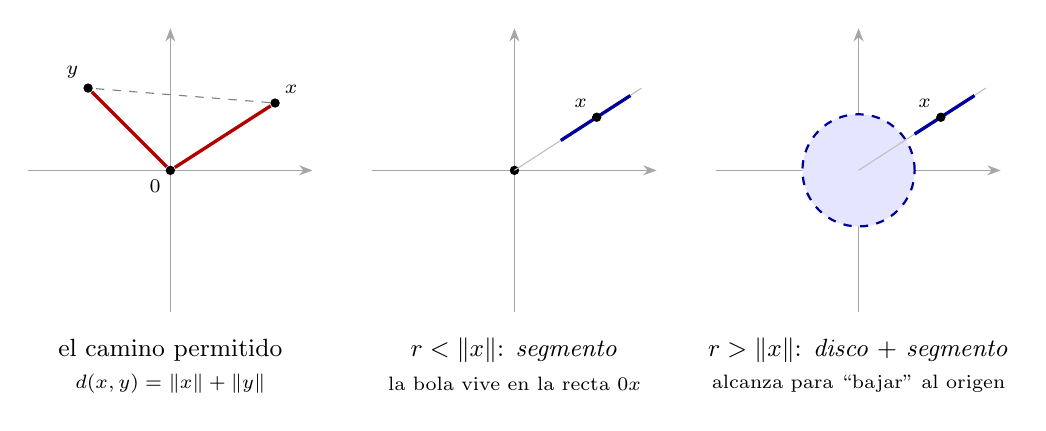
\begin{tikzpicture}[scale=0.95]
% panel 1: como se mide
\begin{scope}
\draw[ejes] (-1.9,0)--(1.9,0); \draw[ejes] (0,-1.9)--(0,1.9);
\node[pt] (O) at (0,0) {}; \node[below left] at (0,0) {\scriptsize $0$};
\node[pt] (x) at (1.4,0.9) {}; \node[above right] at (1.4,0.9) {\scriptsize $x$};
\node[pt] (y) at (-1.1,1.1) {}; \node[above left] at (-1.1,1.1) {\scriptsize $y$};
\draw[red!70!black,very thick] (x)--(O)--(y);
\draw[gray,dashed] (x)--(y);
\node at (0,-2.4) {\small el camino permitido};
\node at (0,-2.85) {\scriptsize $d(x,y)=\|x\|+\|y\|$};
\end{scope}
% panel 2: bola que no contiene al origen
\begin{scope}[xshift=4.6cm]
\draw[ejes] (-1.9,0)--(1.9,0); \draw[ejes] (0,-1.9)--(0,1.9);
\node[pt] at (0,0) {};
\draw[gray!50] (0,0)--(1.7,1.1);
\draw[blue!60!black,very thick] (0.62,0.40)--(1.55,1.0);
\node[pt] at (1.1,0.71) {}; \node[above left] at (1.1,0.71) {\scriptsize $x$};
\node at (0,-2.4) {\small $r<\|x\|$: \emph{segmento}};
\node at (0,-2.85) {\scriptsize la bola vive en la recta $0x$};
\end{scope}
% panel 3: bola que contiene al origen
\begin{scope}[xshift=9.2cm]
\draw[ejes] (-1.9,0)--(1.9,0); \draw[ejes] (0,-1.9)--(0,1.9);
\draw[abierto,dashed] (0,0) circle (0.75);
\draw[gray!50] (0,0)--(1.7,1.1);
\draw[blue!60!black,very thick] (0.75,0.485)--(1.55,1.0);
\node[pt] at (1.1,0.71) {}; \node[above left] at (1.1,0.71) {\scriptsize $x$};
\node at (0,-2.4) {\small $r>\|x\|$: \emph{disco $+$ segmento}};
\node at (0,-2.85) {\scriptsize alcanza para ``bajar'' al origen};
\end{scope}
\end{tikzpicture}
\figtit{Figura 2. Métrica radial (``del ferrocarril''): todos los viajes pasan por el origen, salvo entre puntos de un mismo rayo. Las bolas ya no son redondas ni convexas.}
\end{figure}

\begin{intuicion}
Pensalo como un sistema ferroviario con una única estación central: para ir de un pueblo a otro hay que volver a la capital, salvo que ambos estén sobre la misma vía. Este ejemplo sirve de vacuna contra la idea de que ``bola'' significa ``redondo''. Todo lo que se demuestra usando la palabra \emph{bola} vale también acá; todo lo que se demuestra dibujando un círculo, no.
\end{intuicion}

\begin{ejercicio}[Axiomática mínima \fnt{EJ, Métricos--A.6, p.\,2}]
$d:X\times X\to\R$ es una distancia si y sólo si verifica:
\[
\text{(i) } d(x,y)=0\iff x=y, \qquad
\text{(ii) } d(x,y)\le d(x,z)+d(y,z)\quad \forall x,y,z .
\]
\end{ejercicio}

\begin{proof}
Solo falta ver que (i)+(ii) implican simetría y positividad. Tomando $z=x$ en (ii): $d(x,y)\le d(x,x)+d(y,x)=d(y,x)$, e intercambiando $x$ e $y$ se obtiene la otra desigualdad, luego $d(x,y)=d(y,x)$. Tomando ahora $z=y$ y usando la simetría recién probada: $0=d(x,x)\le d(x,y)+d(x,y)=2d(x,y)$, o sea $d\ge 0$. Con la simetría, (ii) es exactamente la desigualdad triangular.
\end{proof}

\begin{ejercicio}
Vale la pena registrar la técnica: \emph{especializar} la desigualdad triangular en $z=x$ y $z=y$ es el único recurso disponible cuando aún no se dispone de simetría.
\end{ejercicio}

\begin{ejercicio}[¿Cuándo una métrica proviene de una norma? \fnt{EJ, Métricos--A.8, p.\,2}]
Sea $V$ un $\R$-espacio vectorial y $d$ una distancia en $V$. Entonces $d$ proviene de una norma si y sólo si es
\begin{enumerate}[label=(\roman*),leftmargin=2.2em,itemsep=0pt]
\item \emph{invariante por traslaciones}: $d(x+z,y+z)=d(x,y)$ para todos $x,y,z$;
\item \emph{homogénea}: $d(\lambda x,\lambda y)=|\lambda|\,d(x,y)$ para todo $\lambda\in\R$.
\end{enumerate}
En tal caso la norma es $\norm{x}:=d(x,0)$ y se recupera $d(x,y)=\norm{x-y}$.
\end{ejercicio}

\begin{proof}
Si $d(x,y)=\norm{x-y}$, ambas condiciones son inmediatas. Recíprocamente, definiendo $\norm{x}:=d(x,0)$: $\norm{x}=0\iff x=0$ por (iii) de distancia; $\norm{\lambda x}=d(\lambda x,0)=d(\lambda x,\lambda 0)=|\lambda| d(x,0)=|\lambda|\norm{x}$ por homogeneidad; y
\[
\norm{x+y}=d(x+y,0)\le d(x+y,y)+d(y,0)=d(x,0)+d(y,0)=\norm{x}+\norm{y},
\]
usando invariancia por traslaciones en $d(x+y,y)=d(x,0)$. Finalmente $\norm{x-y}=d(x-y,0)=d(x,y)$.
\end{proof}

\begin{ejercicio}[\fnt{EJ, Métricos--A.9, p.\,2}]
Si $A\cap B\ne\emptyset$ entonces $d(A,B)=0$, pero la recíproca es falsa: en $\R$, $A=(0,1)$ y $B=(1,2)$ son disjuntos con $d(A,B)=0$. Con la métrica discreta, en cambio, $d(A,B)=0\iff A\cap B\ne\emptyset$ y $\delta(A)=1$ si $A$ tiene al menos dos puntos \fnt{EJ, Métricos--C.7, p.\,5}.
\end{ejercicio}

\section{Ejercicio teórico N$^\circ$1 --- producto interno}

\begin{ejercicio}[\fnt{EJ, Ej.\ teórico N$^\circ$1.3, p.\,3}]
En $\mathcal{M}_{n\times n}(\R)$, $(A,B)=\operatorname{traza}(AB^{t})$ es producto interno y su norma asociada es la de Frobenius $\norm{A}=\big(\sum_{i,j}a_{ij}^2\big)^{1/2}$. En $C[a,b]$, $(f,g)=\int_a^b f g$ con $\norm{f}=\big(\int_a^b f^2\big)^{1/2}$.
\end{ejercicio}

\begin{ejercicio}[\fnt{EJ, Ej.\ teórico N$^\circ$1.5, p.\,3}]
$\norm{\cdot}_{\text{taxi}}$ en $\R^2$ no proviene de un producto interno: con $u=(1,0)$, $v=(0,1)$ es $\norm{u+v}^2+\norm{u-v}^2=4+4=8$, mientras que $2\norm{u}^2+2\norm{v}^2=4$. Lo mismo sirve con $\norm{\cdot}_{\max}$.
\end{ejercicio}

\section{Guía de espacios métricos --- C}

\begin{ejercicio}[Truncamiento a nivel $r$ \fnt{EJ, Métricos--C.3, p.\,4}]
Dado $(X,d)$ y $r>0$, $d_r(x,y)=d(x,y)$ si $d(x,y)<r$ y $d_r(x,y)=r$ si $d(x,y)\ge r$ es una distancia. (Es el Lema de deformación con $f(t)=\min\{t,r\}$.)
\end{ejercicio}

\begin{ejercicio}[Bolas en la métrica discreta \fnt{EJ, Métricos--C.4, p.\,4}]
En $(\R^3,d_D)$:
\begin{lista}
\item $\Bola{x}{1/2}=\{x\}$;
\item $\Bola{x}{1}=\{x\}$;
\item $\Bola{x}{2}=\R^3$;
\item $\Bolac{x}{1/2}=\{x\}$;
\item $\Bolac{x}{1}=\R^3$.
\end{lista} Notar que $\cl{\Bola{x}{1}}=\{x\}\subsetneq \Bolac{x}{1}=\R^3$; es el contraejemplo estándar de que la clausura de la bola abierta \emph{no} es en general la bola cerrada.
\end{ejercicio}

\begin{ejercicio}[Acotación \fnt{EJ, Métricos--C.5, C.6, C.8, pp.\,4--5}]
Sea $(X,d)$ y $A\subseteq X$ no vacío y acotado. Entonces:
\begin{enumerate}[label=(\roman*),leftmargin=2.2em,itemsep=0pt]
\item existen $x_0\in X$ y $r>0$ con $A\subseteq \Bolac{x_0}{r}$, y de hecho esto vale para \emph{cualquier} $x\in X$ con un radio $r'$ adecuado;
\item si $A\subseteq B$ entonces $\delta(A)\le\delta(B)$, y $\delta(\Bola{x_0}{r})\le 2r$ (la igualdad puede fallar: en la métrica discreta con $r=3$, $\delta=1$);
\item la unión \emph{finita} de acotados es acotada (para uniones infinitas es falso: $\bigcup_n [0,n]=[0,\infty)$).
\end{enumerate}
\end{ejercicio}

\begin{ejercicio}[Convexidad de las bolas en espacios normados \fnt{EJ, Métricos--C.11, p.\,5}]
En $(\R^n,\norm{\cdot})$, $\Bola{x}{r}$ y $\Bolac{x}{r}$ son convexas.
\end{ejercicio}

\begin{proof}
Si $y,z\in\Bola{x}{r}$ y $t\in(0,1)$, sea $w=ty+(1-t)z$. Entonces
\[
\norm{w-x}=\norm{t(y-x)+(1-t)(z-x)}\le t\norm{y-x}+(1-t)\norm{z-x}< tr+(1-t)r=r .
\]
Se usan solo la desigualdad triangular y la homogeneidad, o sea: es una propiedad de la \emph{norma}, no de la métrica. Por eso falla en las métricas radiales del ejemplo anterior.
\end{proof}

\begin{ejercicio}[Clausura de la bola abierta en normados \fnt{EJ, Métricos--C.12, p.\,5}]
En $(\R^n,\norm{\cdot})$ vale $\cl{\Bola{x}{r}}=\Bolac{x}{r}$.
\end{ejercicio}

\begin{proof}
$\subseteq$ es automático porque $\Bolac{x}{r}$ es cerrada y contiene a $\Bola{x}{r}$. Para $\supseteq$, sea $y$ con $\norm{y-x}=r$ y consideremos $y_t=x+t(y-x)$ con $t\in(0,1)$: es $\norm{y_t-x}=tr<r$, luego $y_t\in \Bola{x}{r}$, y $y_t\to y$ cuando $t\to 1^-$. Por lo tanto $y\in\cl{\Bola{x}{r}}$. El argumento usa la estructura de segmento (convexidad), y por eso el resultado es falso en métricos generales, como muestra la métrica discreta.
\end{proof}

\begin{figure}[ht]
\centering
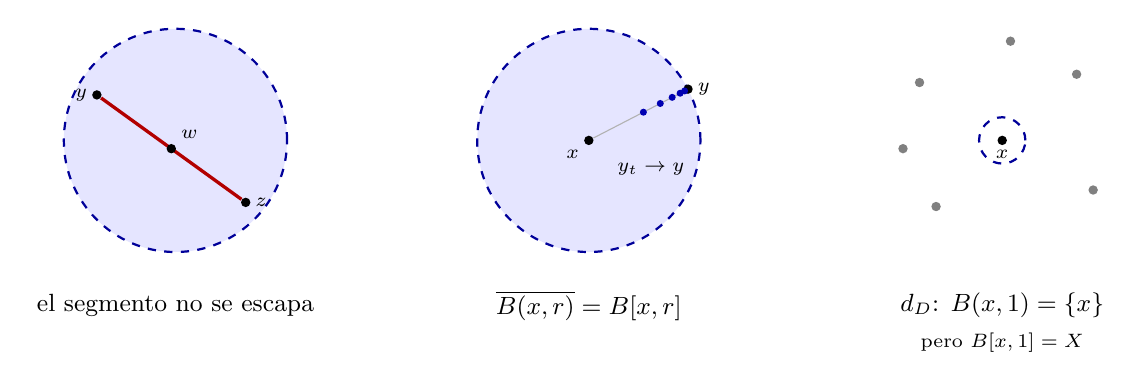
\begin{tikzpicture}[scale=1.05]
% convexidad
\begin{scope}
\draw[abierto,dashed] (0,0) circle (1.35);
\node[pt] (yy) at (-0.95,0.55) {}; \node[left] at (-0.95,0.55) {\scriptsize $y$};
\node[pt] (zz) at (0.85,-0.75) {}; \node[right] at (0.85,-0.75) {\scriptsize $z$};
\draw[red!70!black,very thick] (yy)--(zz);
\node[pt] at (-0.05,-0.1){}; \node[above right] at (-0.05,-0.1) {\scriptsize $w$};
\node at (0,-2.0) {\small el segmento no se escapa};
\end{scope}
% aproximacion a la frontera
\begin{scope}[xshift=5.0cm]
\draw[abierto,dashed] (0,0) circle (1.35);
\node[pt] (c) at (0,0) {}; \node[below left] at (0,0) {\scriptsize $x$};
\node[pt] (yb) at (1.2,0.62) {}; \node[right] at (1.2,0.62) {\scriptsize $y$};
\draw[gray!60] (c)--(yb);
\foreach \t in {0.55,0.72,0.84,0.92,0.965}{
  \node[pt,fill=blue!70!black,inner sep=0.9pt] at ($(c)!\t!(yb)$) {};
}
\node at (0.75,-0.35) {\scriptsize $y_t\to y$};
\node at (0,-2.0) {\small $\cl{\Bola{x}{r}}=\Bolac{x}{r}$};
\end{scope}
% contraejemplo discreto
\begin{scope}[xshift=10.0cm]
\node[pt] at (0,0) {}; \node[below] at (0,0) {\scriptsize $x$};
\foreach \x/\y in {-1.0/0.7,0.9/0.8,1.1/-0.6,-0.8/-0.8,0.1/1.2,-1.2/-0.1}{
  \node[pt,fill=gray] at (\x,\y) {};}
\draw[blue!60!black,thick,dashed] (0,0) circle (0.28);
\node at (0,-2.0) {\small $d_D$: $\Bola{x}{1}=\{x\}$};
\node at (0,-2.45) {\scriptsize pero $\Bolac{x}{1}=X$};
\end{scope}
\end{tikzpicture}
\figtit{Figura 4. Izquierda y centro: en un espacio \emph{normado} las bolas son convexas y la clausura de la abierta es la cerrada. Derecha: en la métrica discreta cada punto está aislado, la bola abierta de radio $1$ es $\{x\}$ y su clausura sigue siendo $\{x\}$, muy lejos de $\Bolac{x}{1}=X$.}
\end{figure}

\begin{intuicion}
Los dos resultados de esta subsección se prueban ``caminando en línea recta'', y en un espacio métrico general no hay líneas rectas: no hay suma ni producto por escalares. Cada vez que una demostración use $tx+(1-t)y$, hay que preguntarse si el enunciado es de espacios \emph{normados} o de espacios \emph{métricos}. La métrica discreta es el test rápido para detectar esa confusión.
\end{intuicion}

\section{Guía de espacios topológicos --- A}

\begin{ejercicio}[Entornos en $\R$ y $\R^2$ euclídeos \fnt{EJ, Top--A.7 y A.8, p.\,6}]
$N$ es entorno de $x$ $\iff$ $N$ contiene un intervalo abierto (resp.\ una bola abierta) centrado en $x$. Así $(-\tfrac12,\tfrac12)$ y $(0,1]$ son entornos de $0$ y de $\tfrac12$ respectivamente, pero $[0,\tfrac12)$ \emph{no} es entorno de $0$ y $(-1,0)$ tampoco (ni siquiera contiene a $0$).
\end{ejercicio}

\begin{ejercicio}[\fnt{EJ, Top--A.10, p.\,7}]
En $(\R,\tp_u)$, con $A=\Q$ y $B=\R-\Q$: $\intr A\cup\intr B=\emptyset$ pero $\intr(A\cup B)=\R$. La inclusión que sí vale en un sentido es coherente con que la unión arbitraria de abiertos es abierta (el miembro izquierdo es un abierto contenido en $A\cup B$, luego está dentro del mayor de ellos).
\end{ejercicio}

\section{Guía de espacios topológicos --- D}

\begin{ejercicio}[Los ejercicios de la guía D, p.\,8]
Los enunciados de la guía D son ejercicios de manipulación fina de $\intr(\cdot)$ y $\cl{(\cdot)}$. Los dos hechos estructurales que conviene tener:
\begin{itemize}[leftmargin=1.4em,itemsep=1pt]
\item Si $A$ es abierto: $A\cap\cl B\subseteq\cl{A\cap B}$ (falso sin la hipótesis de que $A$ sea abierto).
\item \emph{Problema de Kuratowski}: con $i(A)=\intr(\cl A)$ y $c(A)=\cl{\intr A}$ vale $i\circ i=i$ y $c\circ c=c$; a partir de un conjunto se obtienen a lo sumo $7$ conjuntos,
\[
A,\quad \intr A,\quad \cl A,\quad i(A),\quad c(A),\quad i(\intr A),\quad c(\cl A),
\]
con las cadenas $\intr A\subseteq A\subseteq\cl A$, $\ \intr A\subseteq i(\intr A)\subseteq i(A)\subseteq\cl A$ y $\ \intr A\subseteq c(A)\subseteq c(\cl A)\subseteq \cl A$. Ver el Ejemplo~\ref{ej:kur} para un caso donde los siete son distintos.
\item $\fr(A\cup B)\subseteq \fr A\cup \fr B$, con igualdad si $\cl A\cap\cl B=\emptyset$.
\end{itemize}
\end{ejercicio}

\begin{ejercicio}[Los siete conjuntos de Kuratowski, verificados \fnt{EJ, Top--D.2, p.\,8}]\label{ej:kur}
Con la notación del ejercicio, $i(A)=\intr(\cl A)$ y $c(A)=\cl{\intr A}$. En $(\R,\tp_u)$ tomemos
\[
A=(0,1)\ \cup\ (1,2)\ \cup\ \{3\}\ \cup\ \big([4,5]\cap\Q\big).
\]
Cada pedazo cumple un rol: $(0,1)\cup(1,2)$ aporta un agujero interno, $\{3\}$ aporta un punto aislado y $[4,5]\cap\Q$ aporta una parte de interior vacío pero clausura gorda. Calculando en orden:
\[
\begin{array}{r@{\;=\;}l@{\qquad}l}
\intr A & (0,1)\cup(1,2) & \text{ni el 3 ni los racionales son interiores}\\
\cl A & [0,2]\cup\{3\}\cup[4,5] & \text{se rellenan el agujero y los irracionales}\\
i(A)=\intr(\cl A) & (0,2)\cup(4,5) & \text{se perdió el punto aislado 3}\\
c(A)=\cl{\intr A} & [0,2] & \text{se perdieron el 3 y el bloque } [4,5]\\
i(\intr A)=\intr(\cl{\intr A}) & (0,2) & \\
c(\cl A)=\cl{\intr(\cl A)} & [0,2]\cup[4,5] &
\end{array}
\]
Junto con $A$ son siete conjuntos distintos dos a dos. Las cadenas de inclusión son
\[
\intr A\subsetneq A\subsetneq\cl A,\qquad
\intr A\subsetneq i(\intr A)\subsetneq i(A)\subsetneq \cl A,\qquad
\intr A\subsetneq c(A)\subsetneq c(\cl A)\subsetneq\cl A .
\]
En cambio $i(A)$ y $c(A)$ son \emph{incomparables}: $0\in c(A)-i(A)$ y $4{,}5\in i(A)-c(A)$. Ese es el punto del ejercicio: interior y clausura no conmutan, y alternarlas produce genuinamente objetos nuevos --- aunque no infinitos, porque $i\circ i=i$ y $c\circ c=c$ hacen que el proceso se estabilice.
\end{ejercicio}

\begin{figure}[ht]
\centering
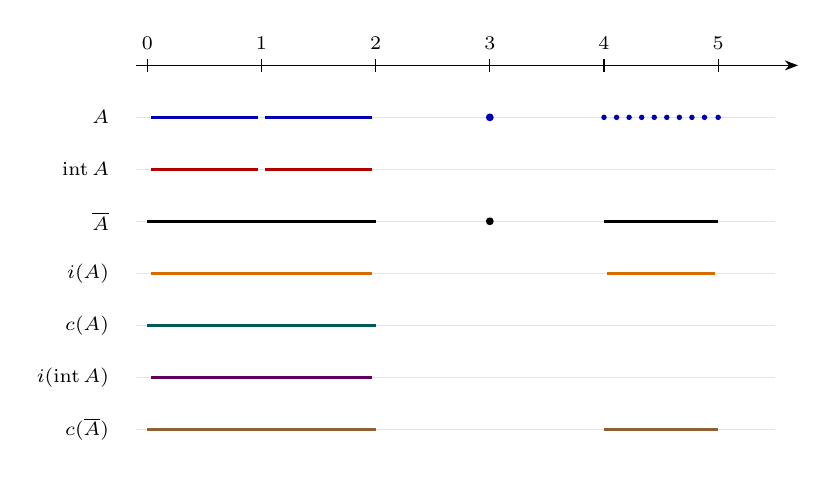
\begin{tikzpicture}[x=1.45cm,y=0.66cm]
\foreach \y in {0,-1,-2,-3,-4,-5,-6}{\draw[gray!22,thin] (-0.1,\y)--(5.5,\y);}
\draw[->,>=Stealth] (-0.1,1)--(5.7,1);
\foreach \x in {0,1,2,3,4,5}{\draw (\x,0.88)--(\x,1.12); \node[above,font=\scriptsize] at (\x,1.12) {$\x$};}
\node[anchor=east,font=\scriptsize] at (-0.25,0) {$A$};
\draw[blue!70!black,very thick] (0.03,0)--(0.97,0);
\draw[blue!70!black,very thick] (1.03,0)--(1.97,0);
\node[pt,fill=blue!70!black,inner sep=1pt] at (3,0) {};
\foreach \x in {4.0,4.11,4.22,4.33,4.44,4.55,4.66,4.77,4.88,5.0}{\node[pt,fill=blue!70!black,inner sep=0.7pt] at (\x,0) {};}
\node[anchor=east,font=\scriptsize] at (-0.25,-1) {$\intr A$};
\draw[red!70!black,very thick] (0.03,-1)--(0.97,-1);
\draw[red!70!black,very thick] (1.03,-1)--(1.97,-1);
\node[anchor=east,font=\scriptsize] at (-0.25,-2) {$\cl A$};
\draw[black,very thick] (0,-2)--(2,-2);
\node[pt,inner sep=1pt] at (3,-2) {};
\draw[black,very thick] (4,-2)--(5,-2);
\node[anchor=east,font=\scriptsize] at (-0.25,-3) {$i(A)$};
\draw[orange!85!black,very thick] (0.03,-3)--(1.97,-3);
\draw[orange!85!black,very thick] (4.03,-3)--(4.97,-3);
\node[anchor=east,font=\scriptsize] at (-0.25,-4) {$c(A)$};
\draw[teal!70!black,very thick] (0,-4)--(2,-4);
\node[anchor=east,font=\scriptsize] at (-0.25,-5) {$i(\intr A)$};
\draw[violet!75!black,very thick] (0.03,-5)--(1.97,-5);
\node[anchor=east,font=\scriptsize] at (-0.25,-6) {$c(\cl A)$};
\draw[brown!75!black,very thick] (0,-6)--(2,-6);
\draw[brown!75!black,very thick] (4,-6)--(5,-6);
\end{tikzpicture}
\figtit{Figura 6b. Los siete conjuntos. Extremos cerrados y abiertos se indican con el trazo lleno hasta el borde o cortado antes; el punto suelto en $3$ y la nube de racionales en $[4,5]$ son los responsables de que todos difieran.}
\end{figure}

\section{Ejercicio teórico N$^\circ$2 --- bases}

\begin{ejercicio}[$K$-topología \fnt{EJ, Ej.\ teórico N$^\circ$2.5, p.\,10; Munkres \S13}]
Sea $K=\{1/n: n\in\N\}$ y $\beta_K=\{(a,b)\}\cup\{(a,b)-K\}$. Es base de una topología $\tp_K$ sobre $\R$ (la \emph{$K$-topología}), \emph{estrictamente} más fina que la usual: $\R-K$ es $\tp_K$-abierto pero no $\tp_u$-abierto, porque ningún intervalo alrededor de $0$ evita a $K$. El criterio de comparación por bases es lo que hace corta esta verificación.
\end{ejercicio}

\begin{figure}[ht]
\centering
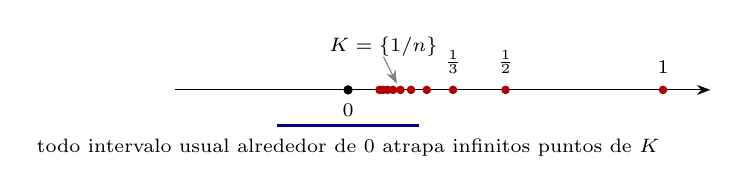
\begin{tikzpicture}[scale=1.0]
\draw[->,>=Stealth] (-2.2,0)--(4.6,0);
\node[pt] at (0,0) {}; \node[below] at (0,-0.05) {\scriptsize $0$};
\foreach \x/\lab in {4/1, 2/\frac12, 1.333/\frac13, 1/\frac14, 0.8/{}, 0.666/{}, 0.571/{}, 0.5/{}, 0.444/{}, 0.4/{}}{
  \node[pt,fill=red!70!black,inner sep=1.1pt] at (\x,0) {};
}
\node[above] at (4,0.08) {\scriptsize $1$};
\node[above] at (2,0.08) {\scriptsize $\frac12$};
\node[above] at (1.333,0.08) {\scriptsize $\frac13$};
\node at (0.45,0.55) {\scriptsize $K=\{1/n\}$};
\draw[->,>=Stealth,gray] (0.45,0.42)--(0.62,0.08);
% intervalo alrededor de 0
\draw[blue!60!black,very thick] (-0.9,-0.45)--(0.9,-0.45);
\node[below] at (0,-0.5) {\scriptsize todo intervalo usual alrededor de $0$ atrapa infinitos puntos de $K$};
\end{tikzpicture}
\figtit{Figura 7. La $K$-topología agrega el abierto $(-1,1)-K$, que contiene a $0$ pero a ningún $1/n$. En la topología usual eso es imposible: $0$ es punto de acumulación de $K$.}
\end{figure}

\begin{intuicion}
Agregar básicos = agregar abiertos = ``romper piedras'' (la imagen de la guía, p.\,9): una topología más fina distingue más puntos. La $K$-topología es lo mínimo que hay que agregarle a $\R$ usual para que $0$ deje de estar pegado a la sucesión $1/n$. Es el ejemplo estándar de dos topologías donde una contiene a la otra \emph{estrictamente}.
\end{intuicion}

\section{Ejercicios teóricos de separación y sucesiones}

\begin{ejercicio}[Límite no único \fnt{EJ, Ej.\ teórico 5b, p.\,11}]
En $(X,\tp_{ind})$ toda sucesión converge a todo punto. En $(\R,\tp_{cof})$, cualquier sucesión de términos distintos dos a dos converge a \emph{todos} los puntos de $\R$: dado $x$ y un abierto $G\ni x$, $\R-G$ es finito, luego contiene a lo sumo finitos términos. Ninguno de los dos es Hausdorff, como debe ser.
\end{ejercicio}

\section{Guía de continuidad --- A}

\begin{ejercicio}[Función característica \fnt{EJ, Continuidad--A.1--A.2, p.\,12}]
Sea $\chi_A:(X,\tp)\to(\R,\tp_u)$. Entonces $\chi_A$ es continua $\iff$ $A$ es simultáneamente abierto y cerrado (equivalentemente, $\fr A=\emptyset$).
\end{ejercicio}

\begin{proof}
Para $U\subseteq\R$ abierto, $\chi_A^{-1}(U)$ solo puede ser $\emptyset$, $A$, $X-A$ o $X$, según si $U$ contiene a $0$, a $1$, a ambos o a ninguno. Luego $\chi_A$ es continua $\iff$ $A$ y $X-A$ son abiertos $\iff$ $A$ es abierto y cerrado. En particular $\chi_\Q:(\R,\tp_u)\to(\R,\tp_u)$ no es continua en ningún punto, porque todo intervalo contiene racionales e irracionales, de modo que la oscilación de $\chi_\Q$ en cualquier entorno es $1$.
\end{proof}

\begin{ejercicio}[$\chi_\Q$ no es continua en ningún punto \fnt{EJ, Continuidad--A.2, p.\,12}]
Sea $a\in\R$ cualquiera y $\varepsilon_0=\tfrac12$. Todo intervalo $(a-\delta,a+\delta)$ contiene racionales e irracionales (densidad de $\Q$ y de $\R-\Q$), luego contiene un punto $x$ con $|\chi_\Q(x)-\chi_\Q(a)|=1\ge\varepsilon_0$. Vía sucesiones: si $a\in\Q$, tomando irracionales $y_n\to a$ es $\chi_\Q(y_n)=0\not\to 1=\chi_\Q(a)$.
\end{ejercicio}

\begin{ejercicio}[Signo \fnt{EJ, Continuidad--A.8, p.\,12}]
$f(x)=x/|x|$ para $x\ne0$ y $f(0)=0$. Es continua en todo $a\ne 0$ (es localmente constante: $f\equiv 1$ en $(a/2,\infty)$ si $a>0$). En $a=0$ no lo es: $x_n=1/n\to0$ da $f(x_n)=1\to 1$ mientras que $y_n=-1/n\to0$ da $f(y_n)=-1$; los dos límites difieren, y ninguno vale $f(0)=0$.
\end{ejercicio}

\begin{ejercicio}[\fnt{EJ, Continuidad--A.4, p.\,12}]
$f:\R^2\to\R^3$, $f(x,y)=(x,x+y,x-y)$ y $f:\R^3\to\R^3$, $f(x,y,z)=(x+y+z,\,xyz)$ (con la coordenada que corresponda) son continuas: cada coordenada es suma o producto de proyecciones, que son continuas, y se aplica el criterio coordenada a coordenada.
\end{ejercicio}

\begin{ejercicio}[Aplicaciones desde topologías ``grandes'' \fnt{EJ, Continuidad--A.5--A.6, p.\,12}]
\begin{enumerate}[label=(\alph*),leftmargin=2.2em,itemsep=0pt]
\item $f:(X,\tp_{cof})\to(X,\tp_{cof})$ con $X$ infinito es homeomorfismo $\iff$ $f$ es biyectiva. (Toda biyección de $X$ preserva la finitud de los complementos, y su inversa también.)
\item Toda $f:(\R,\tp_{conum})\to(\R,\tp_u)$ continua es constante. Idea: si tomara dos valores, se separan por abiertos usuales y se obtienen dos abiertos conumerables disjuntos no vacíos, imposible porque en $\R$ dos conjuntos de complemento numerable siempre se cortan.
\end{enumerate}
\end{ejercicio}

\begin{ejercicio}[Distancia como función continua \fnt{EJ, Continuidad--A.7, p.\,12}]
Sea $(X,d)$ métrico y $d^2_{\max}\big((x_1,x_2),(x_1',x_2')\big)=\max\{d(x_1,x_1'),d(x_2,x_2')\}$ sobre $X\times X$. Entonces $d:(X\times X,d^2_{\max})\to(\R,\tp_u)$ es continua (de hecho $2$-lipschitziana), y nada cambia usando $d_{sum}$ o $d_e$, porque las tres métricas producto son equivalentes.
\end{ejercicio}

\begin{proof}
De la desigualdad triangular cuadrilátera: $|d(x_1,x_2)-d(x_1',x_2')|\le d(x_1,x_1')+d(x_2,x_2')\le 2\,d^2_{\max}$.
\end{proof}

\begin{ejercicio}[\fnt{EJ, Continuidad--A.9, p.\,12}]
Si $f:(\R^n,d_e)\to(\R,d_e)$ es continua, $f^{-1}(a)$ es cerrado para todo $a\in\R$, por ser preimagen del cerrado $\{a\}$. (El mismo argumento muestra que los conjuntos de nivel y las ``curvas implícitas'' $\{f=0\}$ son cerrados.)
\end{ejercicio}

\begin{ejercicio}[Continuidad y densidad \fnt{EJ, Continuidad--A.10, p.\,12}]
Si $D$ es denso en $X$ y $f:(X,\tp)\to(Y,\tp')$ es continua y sobreyectiva, entonces $f(D)$ es denso en $Y$.
\end{ejercicio}

\begin{proof}
$Y=f(X)=f(\cl D)\subseteq\cl{f(D)}$, usando la sobreyectividad y la definición de continuidad por clausuras. Es el argumento donde la definición ``$f(\cl A)\subseteq\cl{f(A)}$'' se paga sola.
\end{proof}

\section{Guía de continuidad --- B}

\begin{ejercicio}[Isometrías \fnt{EJ, Continuidad--B.4, p.\,13}]
Si $f:(X,d)\to(Y,\rho)$ es biyectiva y preserva distancias ($\rho(f(x),f(x'))=d(x,x')$), entonces $f$ es homeomorfismo.
\end{ejercicio}

\begin{proof}
$f$ es continua con $\delta=\varepsilon$; y $f^{-1}$ también preserva distancias (aplicar la igualdad a $f^{-1}(y),f^{-1}(y')$), luego es continua por el mismo argumento.
\end{proof}

\begin{ejercicio}[Conjuntos definidos por desigualdades \fnt{EJ, Continuidad--B.5--B.6, p.\,13}]
Sean $f,g:(X,\tp)\to(\R,\tp_u)$ continuas. Entonces $\{x: f(x)<g(x)\}$ es abierto. Si $f,g:X\to Y$ son continuas con $Y$ Hausdorff, entonces $\{x: f(x)\ne g(x)\}$ es abierto (equivalentemente, $\{x: f(x)=g(x)\}$ es cerrado).
\end{ejercicio}

\begin{proof}
Para el primero: si $f(x_0)<g(x_0)$, elijo $r\in\R$ con $f(x_0)<r<g(x_0)$; entonces
$V=f^{-1}\big((-\infty,r)\big)\cap g^{-1}\big((r,\infty)\big)$ es abierto, contiene a $x_0$ y está contenido en $\{f<g\}$.
Para el segundo: si $f(x_0)\ne g(x_0)$, la condición de Hausdorff da abiertos disjuntos $U\ni f(x_0)$, $V\ni g(x_0)$; entonces $f^{-1}(U)\cap g^{-1}(V)$ es un abierto que contiene a $x_0$, y en cada uno de sus puntos $f$ y $g$ toman valores en conjuntos disjuntos, luego distintos.
\end{proof}

\begin{ejercicio}
La consecuencia clásica: si $f,g$ son continuas en $X$, $Y$ es Hausdorff y $f=g$ sobre un subconjunto \emph{denso}, entonces $f=g$ en todo $X$ (porque $\{f=g\}$ es cerrado y denso).
\end{ejercicio}

\begin{ejercicio}[Dos caminos para $\max\{f,g\}$ \fnt{EJ, Continuidad--B.8, p.\,13}]
Además de la fórmula anterior, hay una demostración puramente topológica que no usa el álgebra y conviene tener a mano porque generaliza: con $h=\max\{f,g\}$,
\[
h^{-1}\big((a,\infty)\big)=f^{-1}\big((a,\infty)\big)\cup g^{-1}\big((a,\infty)\big),
\qquad
h^{-1}\big((-\infty,a)\big)=f^{-1}\big((-\infty,a)\big)\cap g^{-1}\big((-\infty,a)\big),
\]
y ambos son abiertos. Como $\{(a,\infty)\}\cup\{(-\infty,a)\}$ es \emph{subbase} de $\tp_u$, la caracterización de la continuidad por preimágenes de básicos (apunte, Teo.\ 7.5(4)) da la continuidad.
\end{ejercicio}

\begin{ejercicio}[Sobre la guía B.1--B.2, p.\,13]
La continuidad se caracteriza por \emph{preimágenes}, no por imágenes:
\begin{itemize}[leftmargin=1.4em,itemsep=1pt]
\item $f$ es continua $\iff$ $f^{-1}(\intr B)\subseteq \intr\big(f^{-1}(B)\big)$ para todo $B\subseteq Y$;
\item en cambio, ni $f(\intr A)\subseteq\intr(f(A))$ ni $f(\intr A)\supseteq\intr(f(A))$ son necesarias ni suficientes: las funciones que cumplen la primera son las abiertas y no tienen por qué ser continuas (por ejemplo $\R\to\R$ con la identidad en $\Q$ y algo discontinuo fuera), y una constante continua da $f(\intr A)=\{c\}$ mientras $\intr(f(A))=\emptyset$ si $\{c\}$ no es abierto.
\end{itemize}
\end{ejercicio}

%======================================================================
\section{Guía de productos}

\noindent Enunciados de \textbf{TP} p.\,4 (\texttt{01-fuentes/TP-Topologia-Producto.pdf}). Todo producto lleva la topología producto. La técnica común: trabajar en la base de rectángulos y pensar cada rectángulo como intersección de tubos (apunte, \S9).

\begin{ejercicio}[Clausura e interior de un producto \fnt{TP p.\,4, ej.\ 1}]
Si $A\subseteq X$ y $B\subseteq Y$, entonces $\cl{A\times B}=\cl A\times\cl B$ e $\intr(A\times B)=\intr A\times\intr B$.
\end{ejercicio}

\begin{proof}
Es la Prop.\ 9.17 del apunte. Resumen: $\cl A\times\cl B=\pi_X^{-1}(\cl A)\cap\pi_Y^{-1}(\cl B)$ es un cerrado que contiene a $A\times B$ (da $\subseteq$); y si $x\in\cl A$, $y\in\cl B$, todo básico $U\times V\ni(x,y)$ corta a $A\times B$ porque $U$ corta a $A$ y $V$ corta a $B$ (da $\supseteq$). Para el interior: $\intr A\times\intr B$ es un básico dentro de $A\times B$; y si $(x,y)\in U\times V\subseteq A\times B$, entonces $U\subseteq A$ y $V\subseteq B$.
\end{proof}

\begin{ejercicio}[Hausdorff por Hausdorff \fnt{TP p.\,4, ej.\ 2}]
Si $X$ e $Y$ son Hausdorff, $X\times Y$ es Hausdorff.
\end{ejercicio}

\begin{proof}
Apunte, Prop.\ 9.19: dos puntos distintos difieren en una coordenada; se separa esa coordenada con abiertos disjuntos $U_1,U_2$ y se toman los tubos $U_1\times Y$, $U_2\times Y$.
\end{proof}

\begin{ejercicio}[Funciones producto \fnt{TP p.\,4, ej.\ 3}]
(a) Si $f:X\to Z$ y $g:Y\to W$ son continuas, $f\times g:X\times Y\to Z\times W$, $(x,y)\mapsto(f(x),g(y))$, es continua. (b) Si $f:X\to Y$ y $g:X\to Z$ son continuas, $(f,g):X\to Y\times Z$, $x\mapsto(f(x),g(x))$, es continua.
\end{ejercicio}

\begin{proof}
Por el Teorema 9.12 del apunte basta mirar las coordenadas. (a): $\pi_Z\circ(f\times g)=f\circ\pi_X$ y $\pi_W\circ(f\times g)=g\circ\pi_Y$, composiciones de continuas. (b): las coordenadas son $f$ y $g$. Directamente con la base también sale: $(f\times g)^{-1}(U\times V)=f^{-1}(U)\times g^{-1}(V)$ es un rectángulo abierto, y $(f,g)^{-1}(U\times V)=f^{-1}(U)\cap g^{-1}(V)$ es abierto.
\end{proof}

\begin{ejercicio}[Producto menos un rectángulo \fnt{\texttt{Producto-de-Conexos.pdf}, p.\,2}]
Sean $X,Y$ conexos, $A\subsetneq X$ y $B\subsetneq Y$. Entonces $Z=(X\times Y)-(A\times B)$ es conexo.
\end{ejercicio}

\begin{proof}
Como los dos son propios, hay $a_0\in X-A$ y $b_0\in Y-B$. Un punto $(x,y)$ está en $Z$ sii $x\notin A$ o $y\notin B$.
\begin{lista}
\item La cruz $C_0=(\{a_0\}\times Y)\cup(X\times\{b_0\})$ está contenida en $Z$ y es conexa (dos copias conexas de los factores que se cortan en $(a_0,b_0)$; apunte, Prop.\ 10.20).
\item Si $x\notin A$, la vertical $\{x\}\times Y$ está en $Z$, es conexa y corta a $C_0$ en $(x,b_0)$.
\item Si $y\notin B$, la horizontal $X\times\{y\}$ está en $Z$, es conexa y corta a $C_0$ en $(a_0,y)$.
\end{lista}
Entonces $Z$ es la unión de $C_0$ con todas esas verticales y horizontales, cada una de las cuales corta a $C_0$: por la Prop.\ 10.15(a) del apunte (uno que corta a todos), $Z$ es conexo.
\end{proof}

\begin{observacion}[Otra cruz \fnt{\texttt{Producto-de-Conexos.pdf}, p.\,1}]
El apunte de cátedra prueba el producto de conexos con dos cruces, $A=(X\times\{y_1\})\cup(\{x_1\}\times Y)$ y $B=(X\times\{y_2\})\cup(\{x_2\}\times Y)$, que se cortan en $(x_1,y_2)$. En clase alcanzó con una sola cruz, eligiendo una coordenada de cada punto. Las dos versiones valen.
\end{observacion}

%======================================================================
\section{Guía de conexidad}

\noindent Enunciados de \texttt{01-fuentes/Ejercicios-Conexidad-2020.pdf}, citada \textbf{CX}. En clase se pidieron los ejercicios 1 a 10 salvo el 4 (usa Bolzano), con énfasis en 5, 6 y 7. Se resuelven además 11--14, que sólo usan lo dictado. Los 15--23 (arcoconexidad, componentes, conexión local, compacidad) quedan para cuando se dicten. Las referencias numéricas son al apunte compilado, \S10.

\begin{ejercicio}[Un conexo denso hace conexo a lo que lo contiene \fnt{CX 1}]
Si $A\subseteq B\subseteq X$, con $A$ conexo y denso en $X$, entonces $B$ es conexo.
\end{ejercicio}

\begin{proof}
Denso quiere decir $\cl A=X$. Entonces $A\subseteq B\subseteq X=\cl A$ y el sándwich (Prop.\ 10.17) da que $B$ es conexo.
\end{proof}

\begin{ejercicio}[Basta que uno toque la clausura del otro \fnt{CX 2}]
Si $A,B$ son conexos y $\cl A\cap B\ne\emptyset$, entonces $A\cup B$ es conexo.
\end{ejercicio}

\begin{proof}
Sea $C=A\cup(\cl A\cap B)$. Como $A\subseteq C\subseteq\cl A$, $C$ es conexo por el sándwich. Además $C\cap B\supseteq\cl A\cap B\ne\emptyset$, así que $C\cup B$ es conexo (unión de dos conexos que se cortan, Prop.\ 10.14). Y $C\cup B=A\cup B$.
\end{proof}

\begin{observacion}
La hipótesis $A\cap B\ne\emptyset$ se debilitó a $\cl A\cap B\ne\emptyset$. No alcanza con $\cl A\cap\cl B\ne\emptyset$: $(0,1)$ y $(1,2)$ tienen clausuras que se cortan en $1$, y su unión no es conexa.
\end{observacion}

\begin{ejercicio}[Conexo sii nadie propio tiene frontera vacía \fnt{CX 3}]
$X$ es conexo si y sólo si todo $A\subseteq X$ con $A\ne\emptyset$ y $A\ne X$ tiene frontera no vacía.
\end{ejercicio}

\begin{proof}
El enunciado impreso pide sólo $A\ne X$, pero hay que excluir también $A=\emptyset$, cuya frontera siempre es vacía. Por la Prop.\ 3.17, $\fr A=\emptyset$ sii $A$ es abierto y cerrado. Entonces ``ningún $A\ne\emptyset,X$ tiene frontera vacía'' dice ``no hay abiertos-cerrados propios'', que es la conexidad (Prop.\ 10.5).
\end{proof}

\begin{ejercicio}[Bolzano \fnt{CX 4} \noentra{usa los intervalos de $\R$, todavía no dictados}]
$X$ es conexo si y sólo si toda $f:X\to(\R,\tp_e)$ continua que toma un valor negativo y uno positivo se anula.
\end{ejercicio}

\begin{proof}
($\Leftarrow$) Por el contrarrecíproco: si $(U,V)$ desconecta a $X$, la función que vale $-1$ en $U$ y $1$ en $V$ es continua (las preimágenes de abiertos son $\emptyset$, $U$, $V$ o $X$), toma los dos signos y no se anula. ($\Rightarrow$) $f(X)$ es conexo (Prop.\ 10.8) y los conexos de $\R$ son intervalos (GT 4.4.4, pendiente); un intervalo que tiene un número negativo y uno positivo contiene al $0$.
\end{proof}

\begin{ejercicio}[Uniones de familias \fnt{CX 5, 6 y 7}]
Si $\{C_\alpha\}$ son conexos y (5) se cortan dos a dos, o (6) todos cortan a un $C_0$ fijo, o (7) es una sucesión con $C_i\cap C_{i+1}\ne\emptyset$, la unión es conexa.
\end{ejercicio}

\begin{proof}
Es la Prop.\ 10.15, con la demostración indicada en clase: dados $x,y$ en la unión se los mete en un conexo contenido en ella usando la unión de dos (Prop.\ 10.14), y se concluye con la versión para subconjuntos de ``dos puntos en un conexo'' (Prop.\ 10.13). En (5) sirve $C_\alpha\cup C_\beta$; en (6), $C_\alpha\cup C_0\cup C_\beta$; en (7), $C_i\cup\dots\cup C_j$ por inducción.
\end{proof}

\begin{ejercicio}[El gráfico de una continua \fnt{CX 8}]
Si $X$ es conexo y $f:X\to Y$ es continua, el gráfico $G=\{(x,f(x)): x\in X\}$ es conexo en $X\times Y$.
\end{ejercicio}

\begin{proof}
$G$ es la imagen de $h:X\to X\times Y$, $h(x)=(x,f(x))$. Sus coordenadas son $1_X$ y $f$, continuas, así que $h$ es continua (Teo.\ 9.12), y la imagen continua de un conexo es conexa (Prop.\ 10.8).
\end{proof}

\begin{ejercicio}[Conexidad y finura \fnt{CX 9}]
Si $\tp$ es más fina que $\tp'$ ($\tp'\subseteq\tp$): $(X,\tp)$ conexo $\Rightarrow$ $(X,\tp')$ conexo. La recíproca es falsa.
\end{ejercicio}

\begin{proof}
$1_X:(X,\tp)\to(X,\tp')$ es continua (Prop.\ 7.13) y sobreyectiva: la imagen de un conexo es conexa. O directamente: una desconexión de $(X,\tp')$ lo sería también de $(X,\tp)$, que tiene más abiertos. Contraejemplos de la recíproca: $\R$ usual es conexo y $\R$ discreto (o Sorgenfrey, donde $[a,b)$ es abierto y cerrado) no lo es.
\end{proof}

\begin{ejercicio}[La cofinita es conexa \fnt{CX 10}]
Si $X$ es infinito, $(X,\tp_{cof})$ es conexo.
\end{ejercicio}

\begin{proof}
Si $U,V$ fueran abiertos no vacíos y disjuntos, $X=X-(U\cap V)=(X-U)\cup(X-V)$ sería unión de dos conjuntos finitos, luego finito. Absurdo: no hay desconexiones.
\end{proof}

\begin{definicion}[Totalmente disconexo \fnt{CX, p.\,2}]
$X$ es \emph{totalmente disconexo} si para todos $x\ne y$ existen abiertos disjuntos $U\ni x$, $V\ni y$ con $U\cup V=X$.
\lgc{\forall x\ne y\ \exists U,V\in\tp:\ x\in U\ \wedge\ y\in V\ \wedge\ U\cap V=\emptyset\ \wedge\ U\cup V=X.}
\end{definicion}

\begin{ejercicio}[Ejemplos no discretos \fnt{CX 11}]
$\Q$ con la topología usual y la recta de Sorgenfrey son totalmente disconexos.
\end{ejercicio}

\begin{proof}
En $\Q$: si $x<y$, se elige un irracional $r$ entre ellos y se toman $U=(-\infty,r)\cap\Q$ y $V=(r,+\infty)\cap\Q$, que son abiertos, disjuntos y cubren $\Q$ porque $r\notin\Q$. En Sorgenfrey: si $x<y$, se toman $U=(-\infty,y)$ y $V=[y,+\infty)=\bigcup_n[y,y+n)$, ambos abiertos.
\end{proof}

\begin{ejercicio}[Totalmente disconexo $\Rightarrow$ Hausdorff \fnt{CX 12}]
\end{ejercicio}

\begin{proof}
La definición ya da, para $x\ne y$, abiertos disjuntos $U\ni x$, $V\ni y$: eso es $T_2$. (Sobra la condición $U\cup V=X$.)
\end{proof}

\begin{ejercicio}[Sus conexos son los puntos \fnt{CX 13}]
En un totalmente disconexo, los únicos conexos no vacíos son los unitarios.
\end{ejercicio}

\begin{proof}
Si $C$ tuviera dos puntos $x\ne y$, los $U,V$ de la definición lo desconectarían (Prop.\ 10.3): $x\in U\cap C$, $y\in V\cap C$, $U\cap V\cap C=\emptyset$ y $C\subseteq X=U\cup V$.
\end{proof}

\begin{ejercicio}[Un conexo que entra y sale de $B$ toca su frontera \fnt{CX 14}]
Si $A$ es conexo, $A\cap B\ne\emptyset$ y $A\cap(X-B)\ne\emptyset$, entonces $A\cap\fr B\ne\emptyset$.
\end{ejercicio}

\begin{proof}
Por el absurdo, supongamos $A\cap\fr B=\emptyset$. Como $X=\intr B\,\dot\cup\,\fr B\,\dot\cup\,\ext B$, resulta $A\subseteq\intr B\cup\ext B$. Sean $G=\intr B$ y $H=\ext B=\intr(X-B)$, abiertos y disjuntos.
\begin{lista}
\item Si $a\in A\cap B$: $a\notin\fr B$ y $a\notin\ext B\subseteq X-B$, luego $a\in G$. Así $G\cap A\ne\emptyset$.
\item Si $a'\in A-B$: $a'\notin\fr B$ y $a'\notin\intr B\subseteq B$, luego $a'\in H$. Así $H\cap A\ne\emptyset$.
\end{lista}
Con $G\cap H=\emptyset$ y $A\subseteq G\cup H$, la Prop.\ 10.3 dice que $A$ no es conexo. Absurdo.
\end{proof}

\begin{intuicion}
Es la versión topológica de ``para cruzar de adentro hacia afuera hay que pasar por el borde''. En $\R$ con $A$ un intervalo, es el teorema del valor intermedio.
\end{intuicion}

\begin{ejercicio}[Peine del topólogo \fnt{\texttt{Peine-del-Topologo.pdf}} \noentra{usa que $[0,1]$ es conexo; la arcoconexidad no está dictada}]
Sea $K=\{1/n: n\in\N\}$. El \emph{peine} $P=(\{0\}\times[0,1])\cup(K\times[0,1])\cup([0,1]\times\{0\})\subseteq\R^2$ es conexo, y el \emph{peine reducido} $R=\{(0,1)\}\cup(K\times[0,1])\cup([0,1]\times\{0\})$ también.
\end{ejercicio}

\begin{proof}
Sea $E=(K\times[0,1])\cup([0,1]\times\{0\})$. Cada diente $\{1/n\}\times[0,1]$ y la base $[0,1]\times\{0\}$ son conexos (homeomorfos a $[0,1]$), y todos los dientes cortan a la base: $E$ es conexo por la Prop.\ 10.15(a). Su clausura es $P$: los puntos $(0,t)$ son límites de $(1/n,t)$, y $P$ es cerrado. Como $E\subseteq R\subseteq P=\cl E$ y $E\subseteq P\subseteq\cl E$, el sándwich da que $R$ y $P$ son conexos.
\end{proof}

\begin{observacion}
Según las notas manuscritas de la cátedra, $P$ es además arcoconexo pero no localmente arcoconexo, y $R$ es conexo pero \emph{no} arcoconexo: ningún camino une $(0,1)$ con la base. Es el ejemplo estándar de que conexo no implica arcoconexo. Queda para cuando se dicte arcoconexidad (GT \S\S4.1--4.3).
\end{observacion}

\begin{observacion}[Ejercicios 15--23, pendientes]
Usan temas todavía no dictados: arcoconexidad (15, 16, 17), conexión local (18, 22), componentes conexas (19, 20, 23) y compacidad (21). En el 19 hay que mostrar que $X=\N\cup\bigcup_n(-n-1,-n)$ e $Y=\N\cup[\tfrac12,\tfrac23]\cup\bigcup_n(-n-1,-n)$ no son homeomorfos; se hace contando componentes (GT 4.6.10).
\end{observacion}

\end{document}
